\documentclass[12pt]{article}

% --- Packages ---
\usepackage[utf8]{inputenc}
\usepackage[T1]{fontenc}
\usepackage[french]{babel}
\usepackage{amsmath, amssymb}
\usepackage{geometry}
% \usepackage[draft]{graphicx}
\usepackage{tikz}
\usepackage[most]{tcolorbox}
\usepackage{multicol}
\usepackage{lmodern}
\usepackage{pgfplots}
\pgfplotsset{compat=1.18}
\usepackage{mdframed}
\usepackage{tkz-tab}
\usepackage{bm}
\usepackage{xcolor}
\usepackage{sectsty}
\usepackage[utf8]{inputenc}
\usepackage[T1]{fontenc}
\usepackage[inline]{enumitem}
\usepackage[dvipsnames]{xcolor}
\usepackage{multido}
% --- Page ---
\geometry{margin=2cm}

% Footer
\usepackage{fancyhdr}
\pagestyle{fancy}
\cfoot{\thepage}
\rfoot{\textit{G.M.}}
\renewcommand{\headrulewidth}{0pt}
\renewcommand{\footrulewidth}{0pt}

% Pour les normes : 
\newcommand*{\norme}[1]{\left\lVert\overrightarrow{#1}\right\rVert}

\usetikzlibrary{shapes.misc}

\tikzset{cross/.style={cross out, draw=black, minimum size=2*(#1-\pgflinewidth), inner sep=0pt, outer sep=0pt},
%default radius will be 1pt. 
cross/.default={4pt}}

% mettre dans le préambule, après \usepackage{xcolor}
\usepackage{sectsty} % gère facilement la couleur des titres
\setlength{\parindent}{0pt}

\sectionfont{\color{red}\Large\bfseries}     % pour \section*
\subsectionfont{\color{red}\large\bfseries\hspace{1cm}}

\begin{document}

% ============================
%   Probabilités conditionnelles
% ============================

\newpage

\begin{center}
    {\LARGE \textbf{Probabilités conditionnelles}}\\[4mm]
    {\large Seconde}
\end{center}

\hrule
\vspace{0pt}

% ============================
%   PARTIE 1 : Calculs à l'aide d'un tableau croisé
% ============================

\section*{\textcolor{red}{Partie 1 : Calculs à l'aide d'un tableau croisé}}

\vspace{5pt}

\begin{mdframed}[
    linewidth=1pt,
    linecolor=ForestGreen,
    innertopmargin=10pt,
    innerbottommargin=10pt
]
{\color{ForestGreen}\textbf{\underline{Définition :}}}  

On appelle \textbf{probabilité conditionnelle de $\bm{B}$ sachant $\bm{A}$}, la probabilité que l'événement $B$ se
réalise sachant que l'événement $A$ est réalisé. 

\vspace{5pt}
On la note : $P_A(B)$.

\end{mdframed}

{\color{red}\bf{\underline{Exemple et méthode :}}}

\vspace{5pt}
\hspace{1cm}Un laboratoire pharmaceutique a réalisé des tests sur 800 patients atteints d’une maladie.

\vspace{5pt}
Certains sont traités avec le médicament A, d’autres avec le médicament B. 

\vspace{5pt}
Le tableau
présente les résultats de l’étude :

\begin{center}
    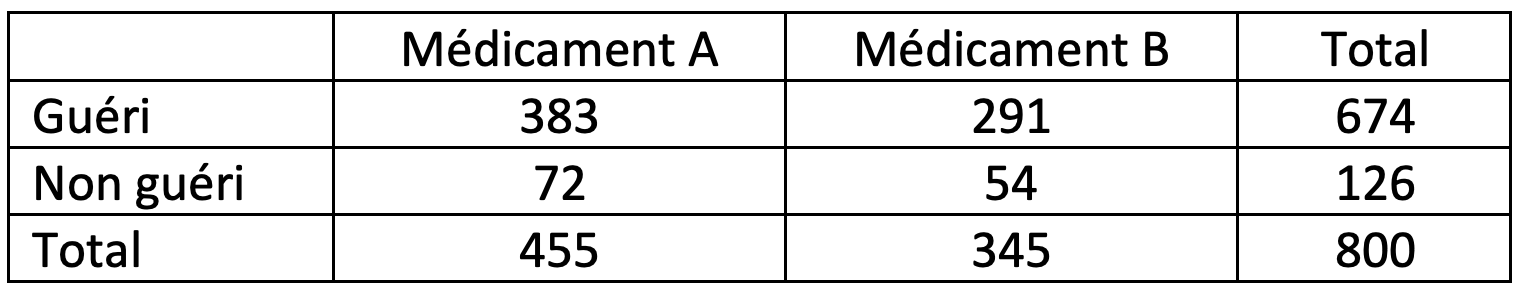
\includegraphics[width=0.6\textwidth]{exemple1.png}
\end{center}

\vspace{5pt}
On choisit au hasard un patient et on considère les évènements suivants :

\vspace{5pt}
\hspace{1cm}$A$ : « Le patient a pris le médicament A. »

\hspace{1cm}$G$ : « Le patient est guéri. »

\vspace{5pt}
\textbf{1) Calculer :}

\vspace{5pt}
\hspace{1cm}a) $P(A)$ \hspace{1cm}b) $P(G)$ 
\hspace{1cm}c) $P(G \cap A)$ \hspace{1cm}d) $P(\bar{G} \cap A)$

\vspace{10pt}
On commence par traduire les évènements en phrase de français :

\begin{itemize}
    \item $A$ : 
    \vspace{10pt}
    \item $G$ : 
    \vspace{10pt}
    \item $G \cap A$ : 
    \vspace{10pt}
    \item $\bar{G} \cap A$ : 
\end{itemize}

\vspace{10pt}
Puis on calcule les probabilités correspondantes : 

\begin{itemize}
    \vspace{10pt}
    \item $P(A) = $
    \vspace{10pt}
    \item $P(G) = $ 
    \vspace{10pt}
    \item $P(G \cap A) = $
    \vspace{10pt}
    \item $P(\bar{G} \cap A) = $
\end{itemize}

\vspace{10pt}
\textbf{2) a) On choisit maintenant au hasard un \underline{patient guéri}.
\\Calculer la probabilité que le patient ait pris le médicament A \underline{sachant qu}'il est guéri.}

\vspace{5pt}
Il faut s'aider du tableau et repérer les lignes/colonnes qui nous intéressent.

\begin{center}
    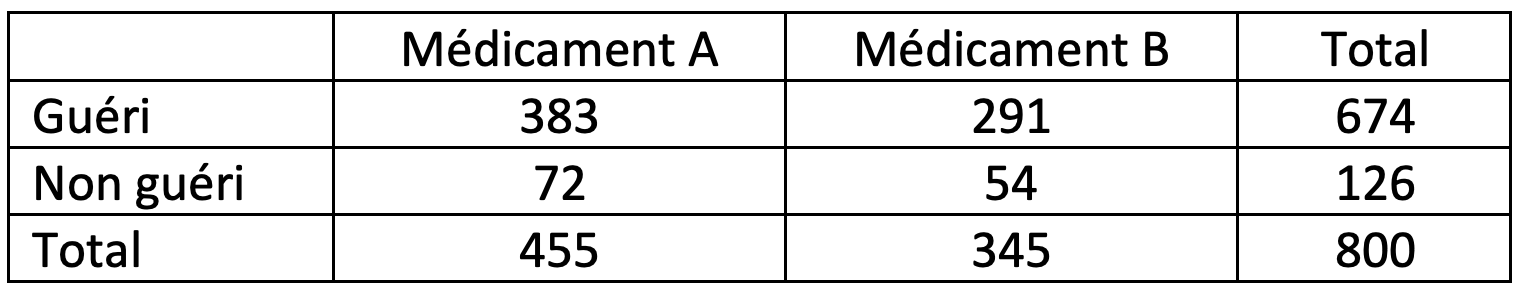
\includegraphics[width=0.6\textwidth]{exemple1.png}
\end{center}

On traduit ensuite en formule la phrase : 

« la probabilité que le patient ait pris le médicament A \underline{sachant qu}'il 
est guéri » : {\color{black!30}\dotfill}

\vspace{5pt}
Et on calcule cette probabilité : 

\vspace{0.5cm}
{\color{black!30}\dotfill}

\vspace{0.5cm}
{\color{black!30}\dotfill}

\vspace{20pt}
\textbf{b) On choisit maintenant au hasard un \underline{patient traité par le médicament B}.
\\Calculer la probabilité que le patient soit guéri \underline{sachant qu}'il a pris le 
médicament B.}

\vspace{10pt}
On applique la même méthode en s'aidant à nouveau du tableau : 

\begin{center}
    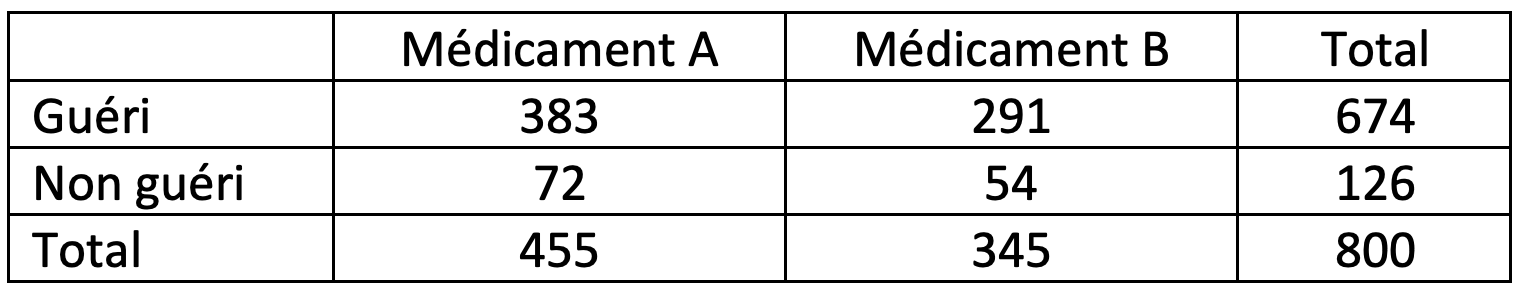
\includegraphics[width=0.6\textwidth]{exemple1.png}
\end{center}

\vspace{0.5cm}
{\color{black!30}\dotfill}

\vspace{0.5cm}
{\color{black!30}\dotfill}

\vspace{0.5cm}
{\color{black!30}\dotfill}

\newpage

\begin{mdframed}[
    linewidth=1pt,
    linecolor=RoyalBlue,
    innertopmargin=10pt,
    innerbottommargin=10pt
]
{\color{RoyalBlue}\textbf{\underline{Exercice d'application n°1 :} 
Calculer des probabilités conditionnelles.}}
\vspace{5pt}

\hspace{1cm} Une urne contient des boules rouges et des boules noires, rayées ou non, 
selon la répartition donnée dans le tableau ci-dessous. 

\vspace{5pt}
On pioche une boule au hasard.

\vspace{-10pt}
\begin{center}
    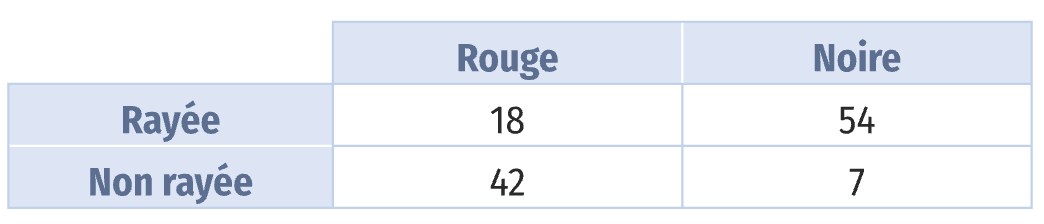
\includegraphics[width=0.6\textwidth]{exercice1.png}
\end{center}

\vspace{-10pt}
\begin{enumerate}
    \item Sachant que la boule tirée est rouge, quelle est la probabilité qu'elle soit rayée ?
    \item Sachant que la boule tirée n'est pas rayée, quelle est la probabilité qu'elle soit noire ?
\end{enumerate}

\vspace{0.5cm}
{\color{black!27}\dotfill}

\vspace{0.5cm}
{\color{black!27}\dotfill}

\vspace{0.5cm}
{\color{black!27}\dotfill}

\vspace{0.5cm}
{\color{black!27}\dotfill}

\vspace{0.5cm}
{\color{black!27}\dotfill}

\vspace{0.5cm}
{\color{black!30}\dotfill}

\vspace{20pt}

{\color{RoyalBlue}\textbf{\underline{Exercice d'application n°2 :} 
Calculer des probabilités conditionnelles.}}

\vspace{5pt}
\hspace{1cm} Lors d'une enquête, on a demandé à 1000 jeunes de 18 à 25 ans s'ils étaient 
titulaires du permis de conduire. Les résultats sont restitués dans le tableau suivant.

\begin{center}
    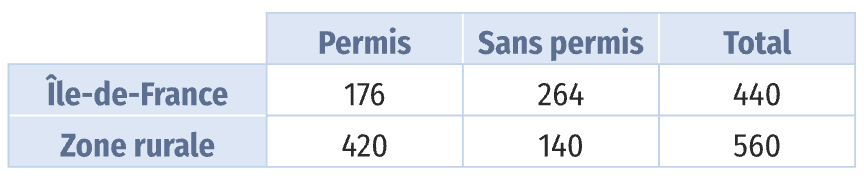
\includegraphics[width=0.6\textwidth]{exercice2.png}
\end{center}

\begin{enumerate}
    \item On interroge au hasard un de ces jeunes d'Île-de- France. Quelle est 
    la probabilité qu'il ait le permis ?
    \item On interroge au hasard un de ces jeunes ayant le permis. Quelle est la probabilité 
    qu'il vienne de zone rurale ? Arrondir à $10^{-2}$ près.
\end{enumerate}

\vspace{0.5cm}
{\color{black!30}\dotfill}

\vspace{0.5cm}
{\color{black!30}\dotfill}

\vspace{0.5cm}
{\color{black!30}\dotfill}

\vspace{0.5cm}
{\color{black!30}\dotfill}

\vspace{0.5cm}
{\color{black!30}\dotfill}

\vspace{0.5cm}
{\color{black!30}\dotfill}

\vspace{0.5cm}
{\color{black!30}\dotfill}

\vspace{20pt}

\end{mdframed}


\vspace{20pt}
% ============================
%   PARTIE 2 : Calculs à l'aide de la formule
% ============================

\section*{\textcolor{red}{Partie 2 : Calculs à l'aide de la formule}}

\vspace{5pt}

\begin{mdframed}[
    linewidth=1pt,
    roundcorner=5pt,
    linecolor=Red,
    innertopmargin=10pt,
    innerbottommargin=0pt
]
{\color{red}
\underline{Propriété :}

\vspace{-10pt}
\[
P_A(B) = \dfrac{Card(A \cap B)}{Card(A)}
\]
}
\end{mdframed}

{\color{red}\textbf{\underline{RAPPEL :}}} $Card(A)$ est le cardinal de $A$, à savoir le \textbf{nombre d'issues 
possibles de l'évènement A}.


\vspace{10pt}
{\color{red}\bf{\underline{Exemple et méthode :}}}

\vspace{5pt}
Un sac contient 50 boules, dont :
\begin{itemize}
    \item 20 boules rouges
    \item 30 boules noires
\end{itemize}
où il est marqué soit "Gagné" ou soit "Perdu".

\begin{itemize}
    \item Sur les 20 boules rouges, 15 sont marquées "Gagné".
    \item Sur les 30 boules noires, 9 sont marquées "Gagné".
\end{itemize}

\vspace{10pt}
\textbf{a) Calculer la probabilité de tirer une boule marquée Gagné sachant qu'elle est rouge.}

\vspace{5pt}
On commence par écrire la formule correspondante à la situation :

\vspace{0.5cm}
{\color{black!30}\dotfill}

\vspace{0.5cm}
{\color{black!30}\dotfill}

\vspace{10pt}
On calcule ensuite les cardinals correspondants :

\begin{minipage}[t]{.45\textwidth}%
    \vspace{10pt}
    % \vspace{pt}
    $Card(R \cap G) = $ {\color{black!30}\dotfill}

    \vspace{20pt}
    $Card(R) = $ {\color{black!30}\dotfill}
\end{minipage}%
\hfill
\begin{minipage}[t]{.45\textwidth}%
    \vspace{0pt}
    
\end{minipage}%

\vspace{10pt}
Et on répond à la question : 

\vspace{0.5cm}
{\color{black!30}\dotfill}

\vspace{0.5cm}
{\color{black!30}\dotfill}

\vspace{20pt}
\textbf{b) Calculer la probabilité de tirer une boule marquée Gagné sachant qu'elle est noire.}

\vspace{5pt}
On applique le même raisonnement pour cette question : 

\vspace{0.5cm}
{\color{black!30}\dotfill}

\vspace{0.5cm}
{\color{black!30}\dotfill}

\vspace{0.5cm}
{\color{black!30}\dotfill}

\vspace{0.5cm}
{\color{black!30}\dotfill}

\vspace{0.5cm}
{\color{black!30}\dotfill}

\vspace{0.5cm}
{\color{black!30}\dotfill}

\vspace{20pt}

\begin{mdframed}[
    linewidth=1pt,
    linecolor=RoyalBlue,
    innertopmargin=10pt,
    innerbottommargin=10pt
]
{\color{RoyalBlue}\textbf{\underline{Exercice d'application n°3 :} 
Calculer des probabilités conditionnelles.}}
\vspace{5pt}

\hspace{1cm} On tire une carte au hasard dans un jeu de 52 cartes. On note R l'événement
« Tirer un cœur ou un carreau » et F l'événement « Tirer une figure ».

\vspace{5pt}
Calculer $P_R(F)$.

\vspace{0.5cm}
{\color{black!27}\dotfill}

\vspace{0.5cm}
{\color{black!27}\dotfill}

\vspace{0.5cm}
{\color{black!27}\dotfill}

\vspace{0.5cm}
{\color{black!27}\dotfill}

\vspace{0.5cm}
{\color{black!27}\dotfill}

\vspace{0.5cm}
{\color{black!30}\dotfill}

\vspace{0.5cm}
{\color{black!30}\dotfill}

\vspace{0.5cm}
{\color{black!30}\dotfill}

\vspace{0.5cm}
{\color{black!30}\dotfill}


\vspace{20pt}

{\color{RoyalBlue}\textbf{\underline{Exercice d'application n°4 :} 
Calculer des probabilités conditionnelles.}}

\vspace{5pt}
\hspace{1cm} On choisit au hasard un fonctionnaire dans une admi- nistration qui en 
compte 65 de catégorie A dont 15 en temps partiel et 85 de catégorie B dont 33 en temps 
partiel. 

\vspace{5pt}
On note A l'événement « La personne choisie est de catégorie A », 

B l'événement « La personne est de catégorie B » 

et C l'événement « La personne choisie travaille à temps complet ».

\begin{enumerate}
    \item Interpréter par une phrase l'événement $A \cap C$.
    \item Interpréter par une phrase l'événement $C$.
    \item Compléter le tableau d'effectifs suivant.
    \begin{center}
        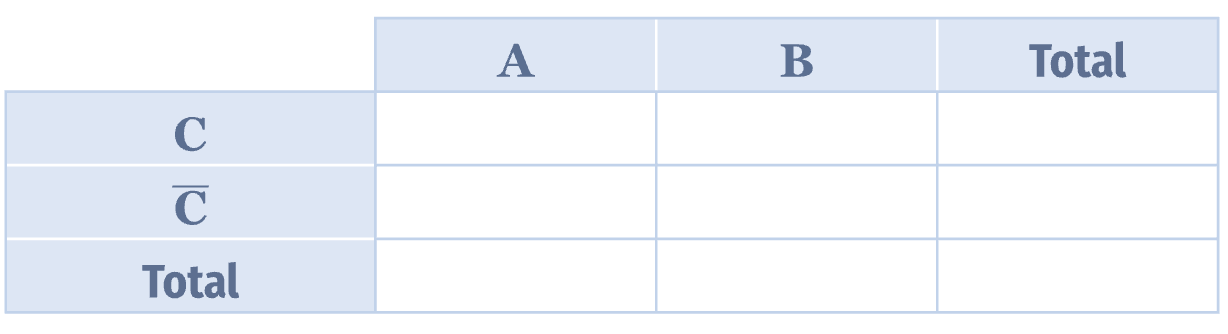
\includegraphics[width=0.8\textwidth]{exercice3.png}
    \end{center}
    \item Calculer la probabilité qu'une personne soit de catégorie B sachant qu'elle est en temps
    partiel.
\end{enumerate}


\vspace{0.5cm}
{\color{black!30}\dotfill}

\vspace{0.5cm}
{\color{black!30}\dotfill}

\vspace{0.5cm}
{\color{black!30}\dotfill}

\vspace{0.5cm}
{\color{black!30}\dotfill}

\vspace{0.5cm}
{\color{black!30}\dotfill}

\vspace{0.5cm}
{\color{black!30}\dotfill}

\vspace{0.5cm}
{\color{black!30}\dotfill}

\vspace{0.5cm}
{\color{black!30}\dotfill}

\vspace{0.5cm}
{\color{black!30}\dotfill}

\vspace{0.5cm}
{\color{black!30}\dotfill}

\vspace{0.5cm}
{\color{black!30}\dotfill}



\vspace{20pt}

\end{mdframed}







\end{document}
